%*----------- SLIDE -------------------------------------------------------------
\begin{frame}[t]{Artigo de Referência} 
    \begin{center}
        \huge 
        Kinematic Modeling and Simulation of a SCARA Robot by Using Solid Dynamics and Verification by
        MATLAB/Simulink\\
        \!
        \\
        \normalsize
        M. S. Alshamasin, F. Ionescu, R. T. Al-Kasasbeh\\
        2009
        
    \end{center}
\end{frame}
%*----------- SLIDE -------------------------------------------------------------
\begin{frame}[c]{Robôs SCARA}
    \framesubtitle{Selective Compliance Articulated Robot Arm} 
    \begin{columns}
        % \column{.01\textwidth}
        \column{.01\textwidth}
        \column{.5\textwidth}

        \begin{figure}
            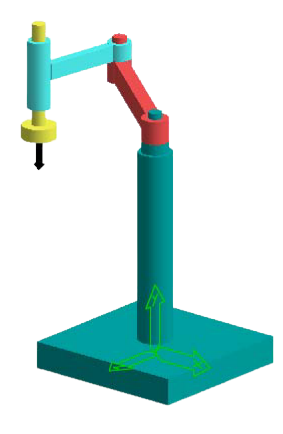
\includegraphics[trim = 0 0 0 0, clip, width=0.5\textwidth]{scara.png}
            %\caption{.}
        \end{figure}

        \column{.49\textwidth}
        \Large
        São robôs manipuladores que possuem:
        \begin{itemize}
            \item Alta velocidade
            \item Alta precisão
            \item 4 graus de liberdade
        \end{itemize}
        % A lei de Zipf pontua a frequência com que certas palavras aparecem nos textos científicos de maneira a definir sua representatividade neste contexto.\\
    \end{columns}
   
%*----------- notes
    \note[item]{Notes can help you to remember important information. Turn on the notes option.}
\end{frame}
\begin{frame}[c]{Aplicações}
    % \begin{figure}
    %     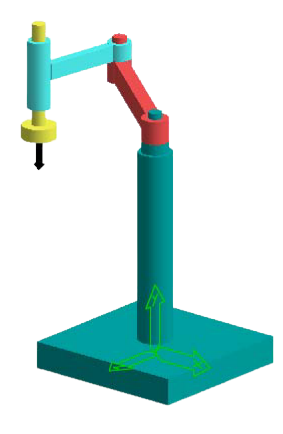
\includegraphics[width=5cm, height=4cm]{scara.png}
    %     %\caption{.}
    % \end{figure}

    \begin{columns}
        % \column{.01\textwidth}
        \column{.01\textwidth}
        \column{.49\textwidth}
        \begin{figure}
            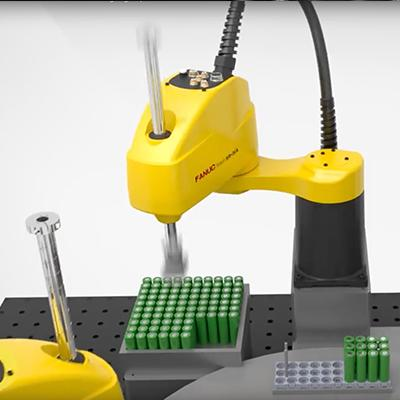
\includegraphics[trim = 0 0 0 0, clip, height=.9\textwidth]{FEA_Speed_assembly-Scara_400x400.jpg}
            %\caption{.}
        \end{figure}    
        % \includemovie{1cm}{1cm}{img07.gif}

        \column{.49\textwidth}
        \begin{figure}
            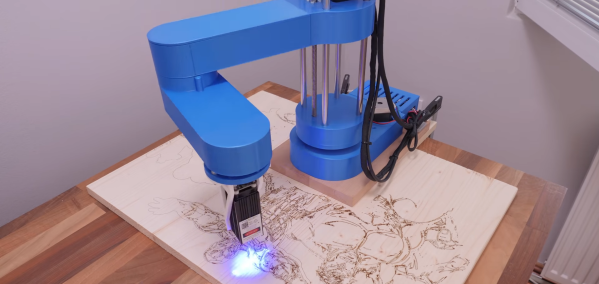
\includegraphics[trim = {5cm 0 5cm 0}, clip, height=.9\textwidth]{2021-08-26-19.png}
            %\caption{.}
        \end{figure}   
        \column{.01\textwidth}
        % A lei de Zipf pontua a frequência com que certas palavras aparecem nos textos científicos de maneira a definir sua representatividade neste contexto.\\
    \end{columns}
%*----------- notes
    \note[item]{Notes can help you to remember important information. Turn on the notes option.}
\end{frame}
%*----------- SLIDE -------------------------------------------------------------
\begin{frame}{Graus de Liberdade}
    \begin{figure}
        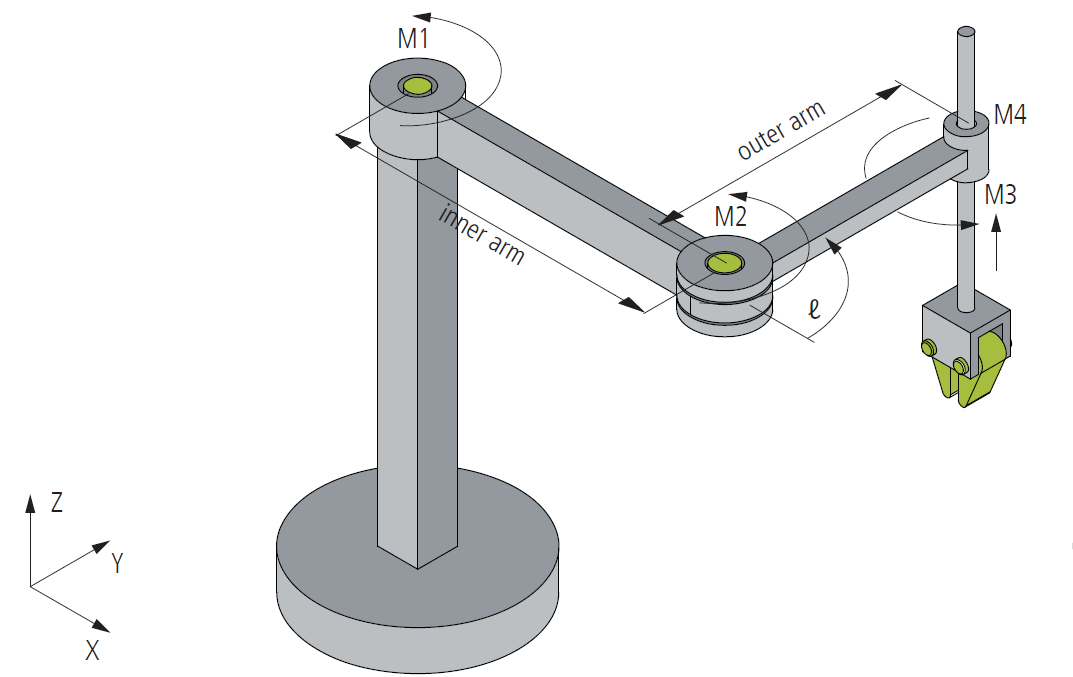
\includegraphics[trim = 160 0 0 0, clip, width=0.6\textwidth]{1232566667__Web.png}
        %\caption{.}
    \end{figure}     
\end{frame}
%*----------- SLIDE -------------------------------------------------------------
\begin{frame}[c]{Modelo Matemático} 
    % \transdissolve[duration=0.5]

    \begin{center}
        \vspace*{1.5cm}
        \textbf{\Huge{Cinemática x Dinâmica}}
    \end{center}
        
    %*----------- notes
    % \begin{center}
    %     \Wider{%
    %     \begin{shaded}
    %     \begin{center}
    %         \vspace*{0.5cm}
    %         \resizebox{!}{0.7cm}{%
    %             \textcolor{cyan}{G}\textcolor{red}{o}\textcolor{orange}{o}\textcolor{cyan}{g}\textcolor{teal}{l}\textcolor{red}{e}?
    %         }%
    %     \end{center}
    %     \end{shaded}
    %     }%
    % \end{center}
%*----------- notes
    \note[item]{Notes can help you to remember important information. Turn on the notes option.}
\end{frame}
%*----------- SLIDE -------------------------------------------------------------
\begin{frame}[c]{Cinemática Direta} 
    \framesubtitle{Notação Denavit-Hartenberg}
    Tem como objetivo obter o conjunto de equações que descreve a cinemática direta de um robô. \\
    Cada junta do robô é descrita através de 4 parâmetros:
    \begin{itemize}
        \item $\theta$ - Ângulo de rotação da junta
        \item d - Deslocamento da junta
        \item a - Comprimento do elo
        \item $\alpha$ - Ângulo de torção da junta
        
    \end{itemize}
    % \centering
    % 
\includegraphics[clip, trim = 0 0 0 0,  width=.83\textwidth]{databases.jpg}
%*----------- notes
    \note[item]{Tem como objetivo pose do end effector a partir dos deslocamentos angulares e lineares das juntas. Pela notação D-H é possível descrever uma junta com 4 parâmetros.}
\end{frame}
%*----------- SLIDE -------------------------------------------------------------
\begin{frame}[c]{Cinemática Direta} 
    \framesubtitle{Notação Denavit-Hartenberg}
    \large
    
    \begin{figure}
        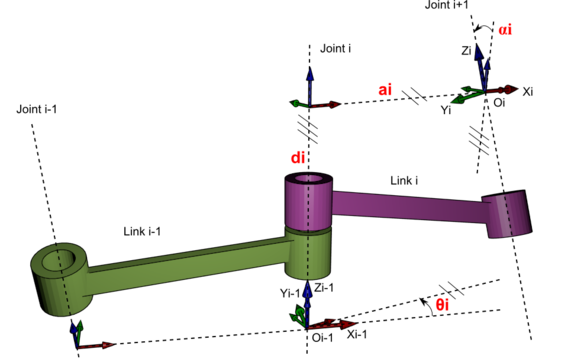
\includegraphics[trim = 0 0 0 0, clip, height=0.4\textwidth]{Classic-DHparameters.png}
    \end{figure}
    % \centering
    % 
\includegraphics[clip, trim = 0 0 0 0,  width=.83\textwidth]{databases.jpg}
%*----------- notes
    \note[item]{Tem como objetivo pose do end effector a partir dos deslocamentos angulares e lineares das juntas. Pela notação D-H é possível descrever uma junta com 4 parâmetros.}
\end{frame}
%*----------- SLIDE -------------------------------------------------------------
\begin{frame}[c]{Cinemática Direta} 
    \framesubtitle{Notação Denavit-Hartenberg}
    \large
    
    \begin{figure}
        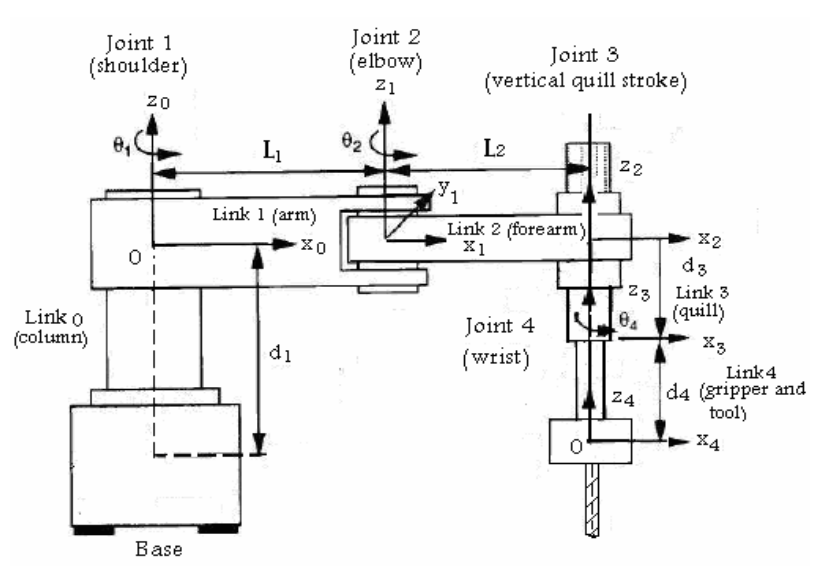
\includegraphics[trim = 0 0 0 0, clip, height=0.4\textwidth]{Screenshot from 2021-11-01 18-11-43.png}
    \end{figure}
    % \centering
    % 
\includegraphics[clip, trim = 0 0 0 0,  width=.83\textwidth]{databases.jpg}
%*----------- notes
    \note[item]{Tem como objetivo pose do end effector a partir dos deslocamentos angulares e lineares das juntas. Pela notação D-H é possível descrever uma junta com 4 parâmetros.}
\end{frame}
%*----------- SLIDE -------------------------------------------------------------
\begin{frame}[c]{Notação Denavit-Hartenberg} 
    % \framesubtitle{Notação Denavit-Hartenberg}
    \large
    
    \begin{figure}
        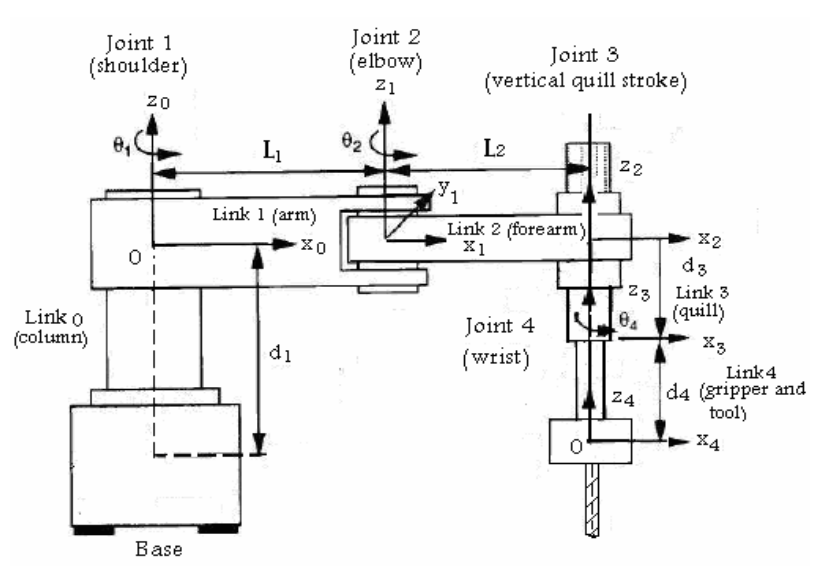
\includegraphics[trim = 0 0 0 0, clip, height=0.35\textwidth]{Screenshot from 2021-11-01 18-11-43.png}
        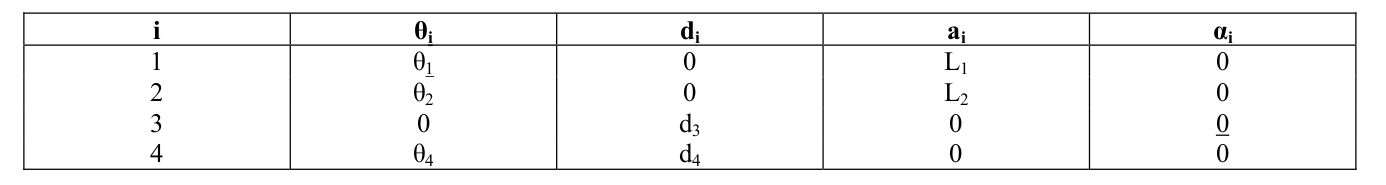
\includegraphics[trim = 0 0 0 0, clip, width=.9\textwidth]{Screenshot from 2021-11-01 18-12-13.png}
    \end{figure}
    % \centering
    % 
\includegraphics[clip, trim = 0 0 0 0,  width=.83\textwidth]{databases.jpg}
%*----------- notes
    \note[item]{Tem como objetivo pose do end effector a partir dos deslocamentos angulares e lineares das juntas. Pela notação D-H é possível descrever uma junta com 4 parâmetros.}
\end{frame}
%*----------- SLIDE -------------------------------------------------------------
\begin{frame}[c]{Notação Denavit-Hartenberg} 
    \framesubtitle{Matriz de Transformação Homogênea}
    \large{
    \begin{itemize}
        \item Matriz de transformação da junta (i-1) e i:\\
        \vspace{0.3cm}
        $T_{i}^{i-1}=Rot(z,\theta_{i})\cdot Trans(z,d_{i})\cdot Trans(x,a_{i})\cdot Rot(x,\alpha_{i})$\\
    \end{itemize}
    
    \begin{itemize}
        \item Matriz de transformação homogênea:\\
        \vspace{0.3cm}
        $T_{n}^{0}=T_{1}^{0}\cdot T_{2}^{1} \cdot T_{3}^{2} \cdots T_{n}^{n-1}$
    \end{itemize}
    }
    % 
\includegraphics[clip, trim = 0 0 0 0,  width=.83\textwidth]{databases.jpg}
%*----------- notes
    \note[item]{Tem como objetivo pose do end effector a partir dos deslocamentos angulares e lineares das juntas. Pela notação D-H é possível descrever uma junta com 4 parâmetros.}
\end{frame}
%*----------- SLIDE -------------------------------------------------------------
\begin{frame}[c]{Cinemática Inversa} 
    % \framesubtitle{Pouco tempo para muito resultado}
    % \transdissolve[duration=0.5]
    Objetivo: Encontrar ângulos e deslocamento angulares das juntas a partir da pose do end effector.
    % \centering
    % 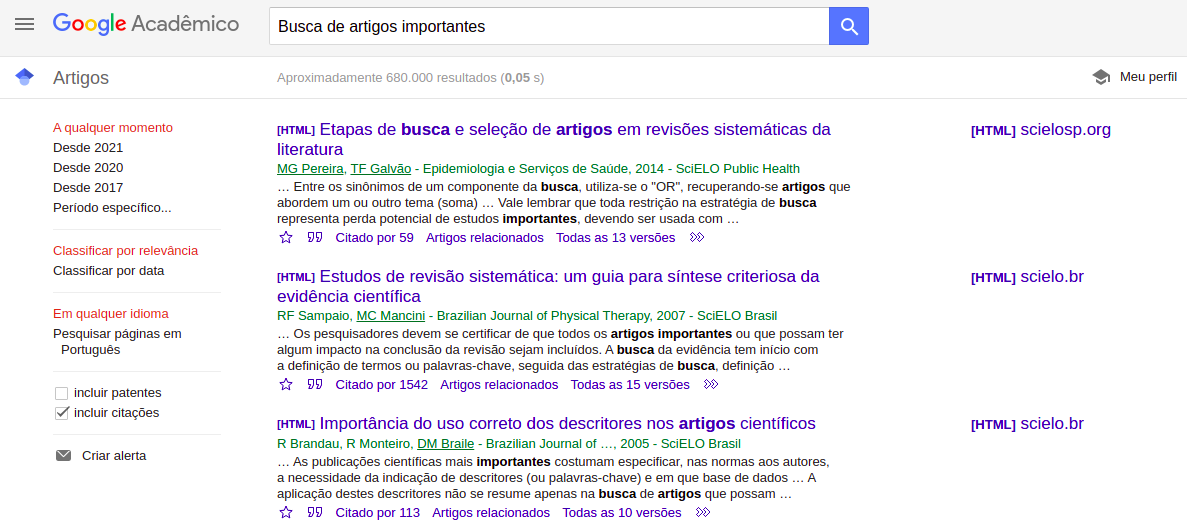
\includegraphics[clip, trim = 0 0 0 0,  width=1\textwidth]{googleacademico2.png}
%*----------- notes
    \note[item]{Notes can help you to remember important information. Turn on the notes option.}
\end{frame}
%-
%*----------- SLIDE -------------------------------------------------------------
\begin{frame}[c]{Como vocês realizam as buscas por artigos?} 
    \framesubtitle{Pouco tempo para muito resultado}
    \transdissolve[duration=0.5]
   
    \centering
    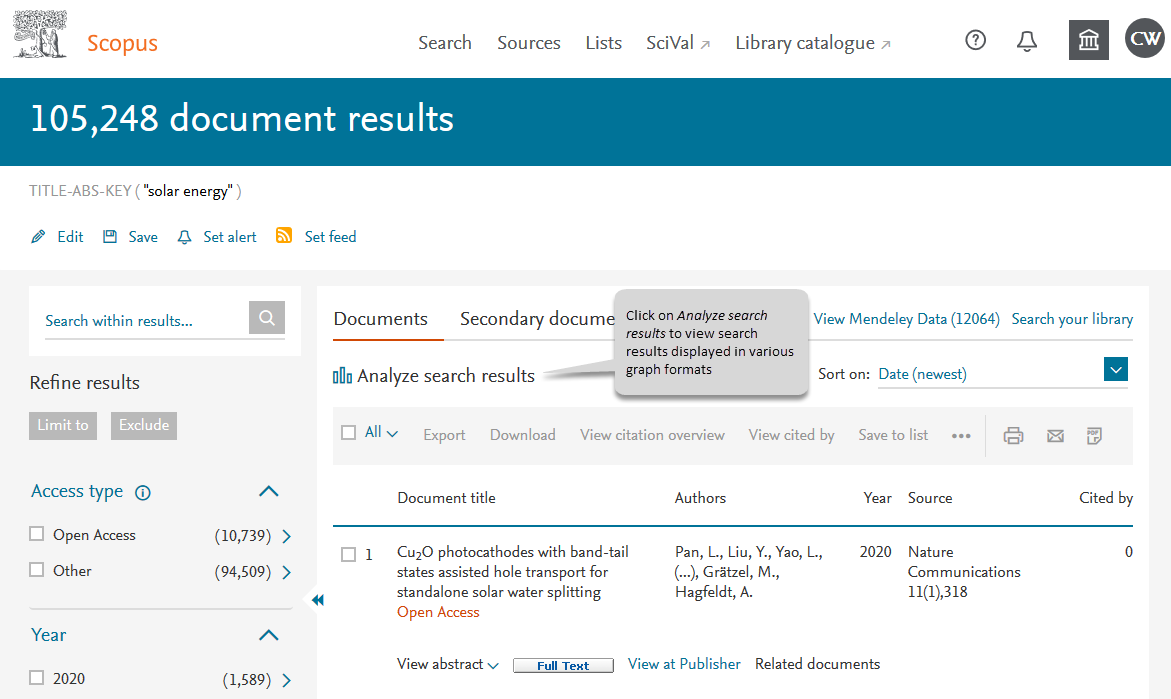
\includegraphics[clip, trim = 0 0 0 0,  width=.75\textwidth]{scopus.png}
%*----------- notes
    \note[item]{Notes can help you to remember important information. Turn on the notes option.}
\end{frame}
%-
%*----------- SLIDE -------------------------------------------------------------
\begin{frame}[c]{Modelo matemático} 
    \framesubtitle{Pouco tempo para muito resultado}
    \transdissolve[duration=0.5]
   
    \centering
    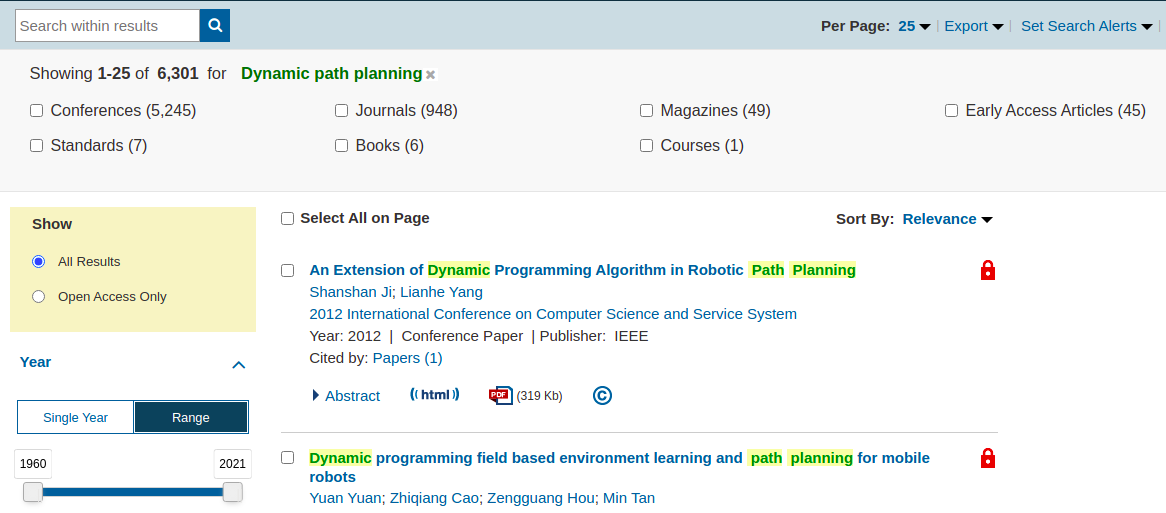
\includegraphics[clip, trim = 0 0 0 0,  width=1\textwidth]{ieee.png}
%*----------- notes
    \note[item]{Notes can help you to remember important information. Turn on the notes option.}
\end{frame}
%-
%*----------- SLIDE -------------------------------------------------------------
\begin{frame}[t]{Tempo e precisão}
    \transboxout[duration=0.5]
    %\framesubtitle{Darwin-OP}
    Uma das vertentes da tecnologia é a capacidade de tornar os processos mais rápidos e precisos, suportando a vida humana no planeta.

    \vspace*{0.2cm}
    Alguns fatores impulsionadores
		\begin{itemize}
			\item Competitividade
			\item Prazo de entrega
			\item Concluir um trabalho 
		\end{itemize}

    \vspace*{0.2cm}
    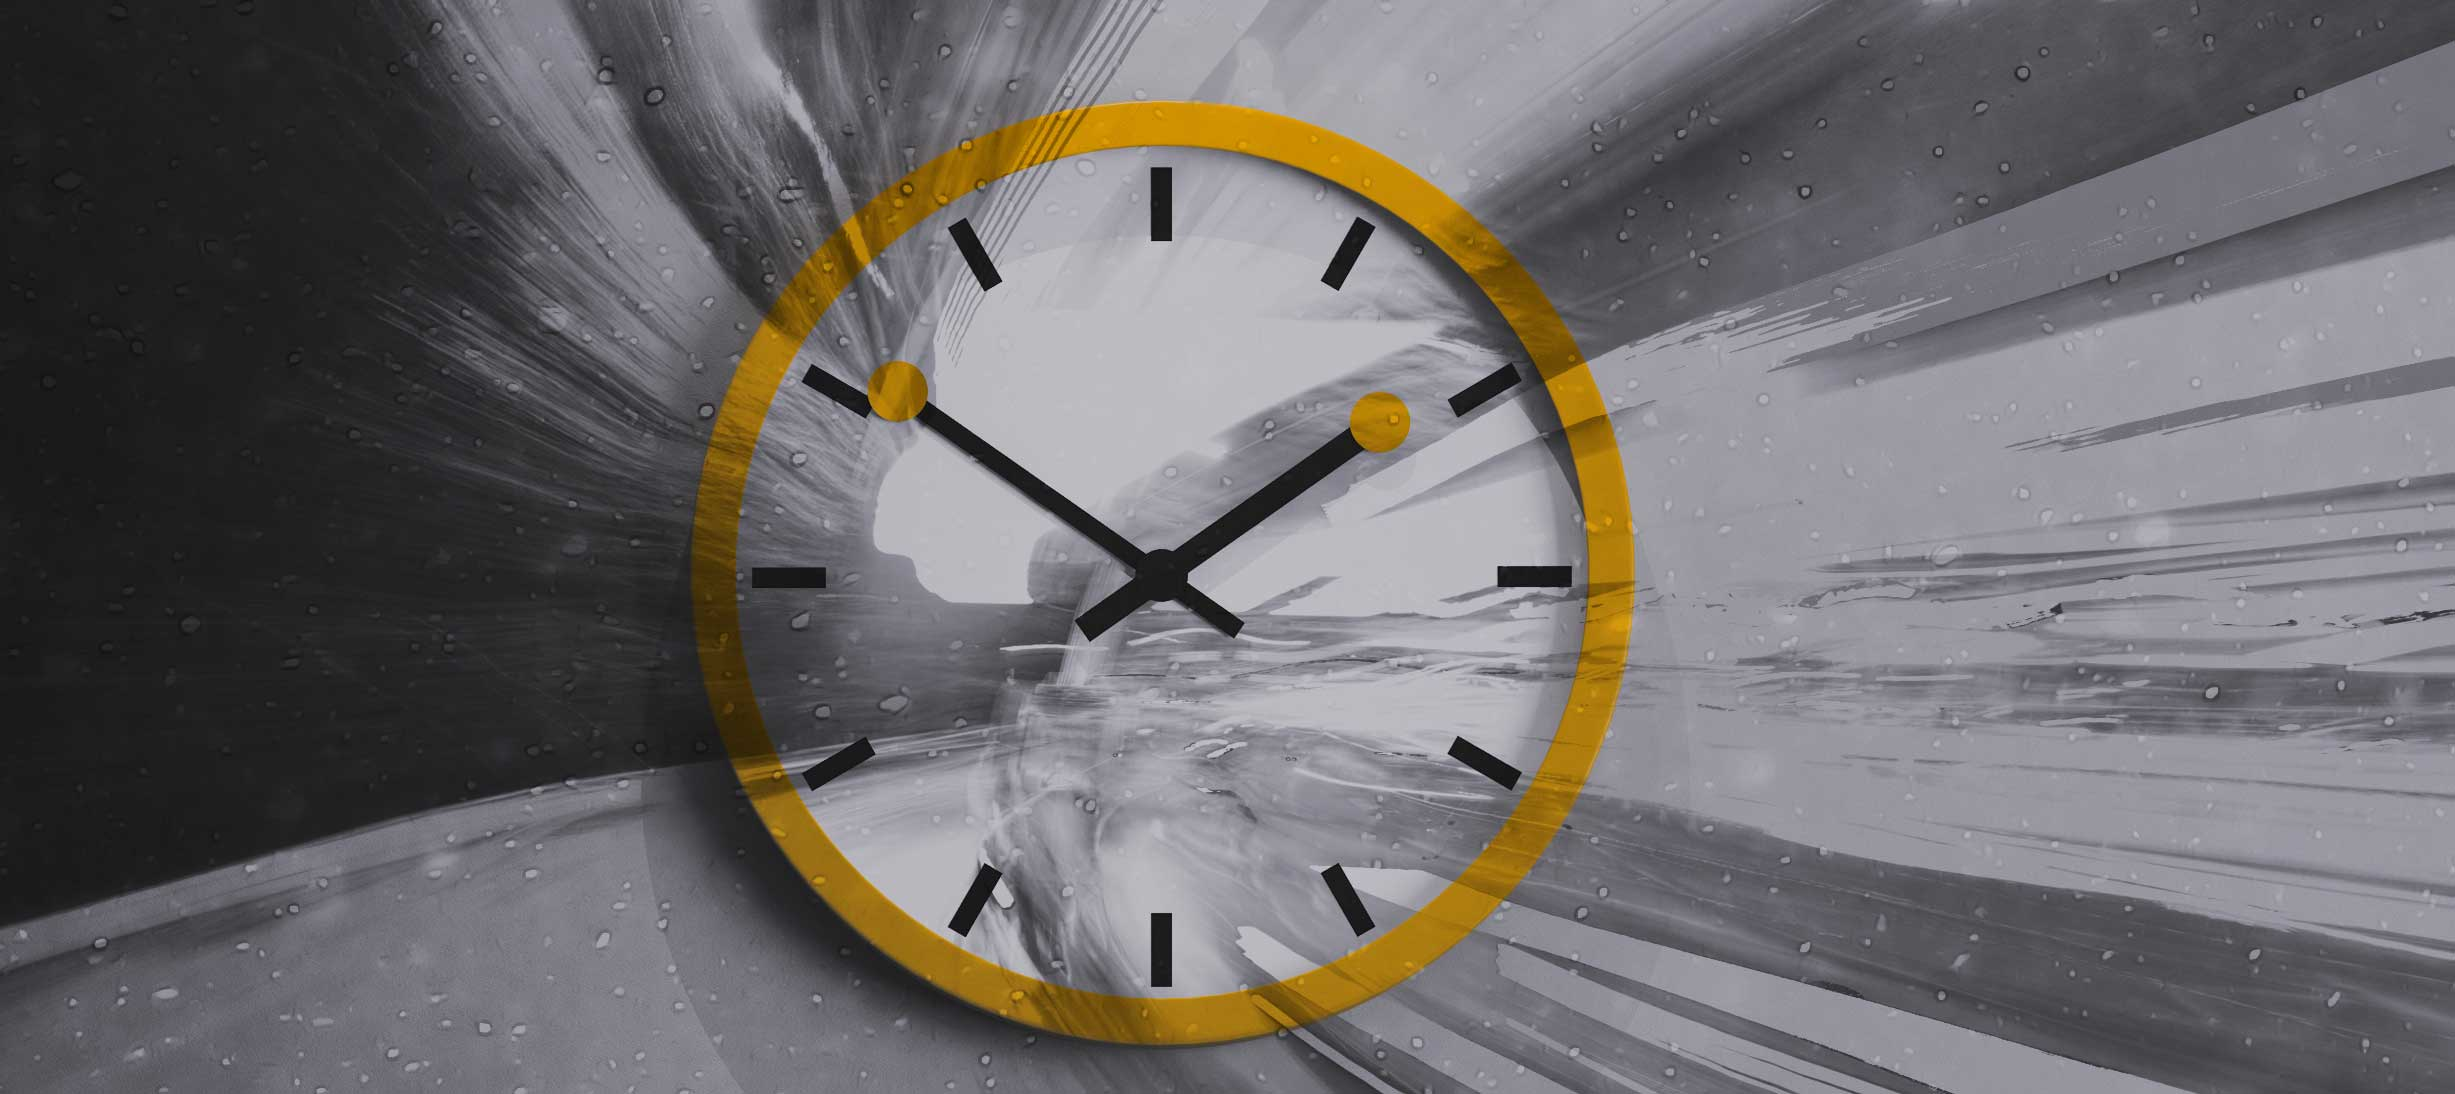
\includegraphics[clip, trim = 0 420 0 80, width=1\textwidth]{time-and-precision.jpeg}

    \begin{columns}
        \column{.1\textwidth}
        \column{.5\textwidth}
        \column{.4\textwidth}
    \end{columns}
%*----------- notes
    \note[item]{Notes can help you to remember important information. Turn on the notes option.}
\end{frame}
%-
